% MIWAI 2026, paper 122. One-page graphical abstract, fourth pass.
%
% v1 grew by accretion: each new block went into whatever space was left, so
% the method band ended up carrying four things and the evidence band three,
% on a grid drawn for three and two. The Grad-CAM pair sat in a gap under the
% frozen branch, four elements in the top band had four different vertical
% anchors, and the lower band stopped 34mm short of the right margin.
%
% v2 fixed the grid. Two things were still wrong. The severity chart was a
% matplotlib import with a rotated axis label, its own legend and nine value
% labels, sitting beside a TikZ chart with none of those, so the two read as
% imports from different documents. And the page carried well over a hundred
% words where the genre asks for under fifty.
%
% So the severity chart is redrawn here in the page's own idiom, as three
% stacked bars rather than nine grouped ones: same numbers, a third of the
% marks, and the Severe sliver reads at the end of each bar. Several notes that
% restated what the layout already shows are gone.
%
% This is a rebuild, not a revision. The previous version was three equal
% rounded cards labelled THE PROBLEM / THE MODEL / THE RESULT. That skeleton is
% the clinical "visual abstract" invented at Annals of Surgery in 2016 for
% tweeting trial results: population, intervention, outcome. It belongs to
% clinical-trial journals talking to a lay audience. This is an AI methods
% paper at an LNAI venue, where the real convention is the CVPR-style teaser
% and the Elsevier single-canvas graphical abstract: one continuous surface,
% no card frames, no chrome, the mechanism drawn rather than asserted.
%
% So: one canvas. The scan anchors it, the pipeline is drawn as a pipeline, and
% the headline sits on an axis next to the baseline it beats, because a number
% on an axis demonstrates and a number in a coloured box only asserts.
%
% Colour is the one deliberate constraint. Radiology is greyscale, so the page
% is greyscale, and the single accent is reserved entirely for the Severe class
% and its recall. Nothing else on the page is coloured. The two branches are
% told apart by solid against dashed, which encodes the actual difference
% (trained against frozen) instead of decorating it.
%
% Type is Charter, a printed-text serif, with Avenir Next Condensed only for
% annotation on and around the image, the way a viewer overlays a scan.
%
% Build (needs lualatex for system fonts):
%   lualatex -interaction=nonstopmode infographic.tex
%   pdftoppm -png -scale-to-x 1920 -scale-to-y 1080 infographic.pdf infographic
% ---------------------------------------------------------------------------
% Fifth pass, 2026-10-03: the advisor's eight points.
%   1 each block now carries a heading set in the page's own type, and the two
%     halves are named "1 Method" and "2 Results" instead of being implied
%   2+7 the comparison is no longer one bar pair: the full four-configuration
%     table from the paper (RSNA Table 3 and SPIDER Table 5) now occupies the
%     right third of the lower half, which is where the two removed footnotes
%     and the old recall chart used to sit
%   3 the two halves are separated by a full-width rule and each is labelled;
%     the right-hand table carries its heading above it, not beside it
%   4 the two provenance lines are gone
%   5+6 the Grad-CAM pair is 48mm instead of 36mm and the scan is 34mm; the
%     page now carries more picture and less prose
%   8 the conference wordmark sits top right above a 13pt paper line, where
%     a 10pt line used to run on alone
% The headline (12.3 to 48.6) moved into the Results heading, so removing the
% bar chart does not cost the one number the page exists to show.
% ---------------------------------------------------------------------------
\documentclass[12pt]{article}
\usepackage[paperwidth=320mm,paperheight=180mm,margin=0mm]{geometry}
\usepackage{fontspec}
\setmainfont{Charter}
\newfontfamily\cond{Avenir Next Condensed}
\usepackage{graphicx}
\usepackage{tikz}
\usetikzlibrary{arrows.meta,positioning,calc,decorations.pathreplacing}
\pagestyle{empty}
\setlength{\parindent}{0pt}

% The first palette used warm, olive-tinted neutrals (F7F7F5, DFDFDA, B8B8B2)
% with a brick accent. Tinted neutrals read as dirty rather than as restrained,
% and the whole page came out dusty. These are clean, faintly cool greys, which
% is what reads as clinical, and the accent now has real chroma.
\definecolor{paper}{HTML}{F8F9FA}
\definecolor{ink}{HTML}{000000}
\definecolor{ink70}{HTML}{34383C}
\definecolor{rule}{HTML}{C9CDD2}
\definecolor{track}{HTML}{E3E7EB}
\definecolor{track2}{HTML}{9AA3AC}
% Matches the Severe red of the paper's own class-distribution figure, so the
% two artefacts agree. Used for the Severe class and its recall, nothing else.
\definecolor{signal}{HTML}{E23B3B}
\definecolor{slot}{HTML}{E3E7EB}
% A second accent, earning its place: it marks everything that is actually
% trained. Blue path against grey dashed frozen blocks is the paper's headline
% about parameter efficiency, drawn instead of stated.
\definecolor{trained}{HTML}{1971C2}
\definecolor{trainedbg}{HTML}{EDF4FC}
\definecolor{bar2}{HTML}{6E7781}
\definecolor{waffle}{HTML}{C3C9CF}
\definecolor{grid}{HTML}{DDE2E6}

\newcommand{\arr}{\raisebox{0.18ex}{\tikz[baseline=-0.55ex]
  \draw[-{Stealth[length=1.9mm,width=1.6mm]},line width=0.5mm](0,0)--(4.4mm,0);}}

\begin{document}
\begin{tikzpicture}[x=1mm,y=1mm,
  box/.style={draw=trained, line width=0.45mm, fill=trainedbg, minimum height=18mm,
              align=center, inner sep=2mm, font=\fontsize{11}{13}\selectfont},
  frz/.style={draw=ink70, line width=0.4mm, dash pattern=on 1.4mm off 1.1mm,
              fill=white, minimum height=18mm, align=center, inner sep=2mm,
              font=\fontsize{11}{13}\selectfont},
  flow/.style={-{Stealth[length=2.2mm,width=1.8mm]}, line width=0.35mm, ink},
  tflow/.style={-{Stealth[length=2.2mm,width=1.8mm]}, line width=0.45mm, trained},
  % Block heading: the advisor's first point. Set in the serif at 13pt so it
  % outranks the 10pt condensed captions without becoming a second title.
  blk/.style={anchor=base west, text=ink, font=\fontsize{13}{15}\selectfont},
  cpt/.style={anchor=base west, text=ink70, font=\cond\fontsize{10}{12}\selectfont}]

\fill[paper] (0,0) rectangle (320,180);

%% ------------------------------------------------------------- title
\node[anchor=base west, font=\fontsize{25}{28}\selectfont]
     at (16,167) {A Two-Branch Hybrid Model for Lumbar Disc Grading};
\node[anchor=base west, text=ink70, font=\fontsize{11}{13}\selectfont]
     at (16,158) {Ha Trung Kien and Phan Trong Nhan, Ho Chi Minh City University of Technology, Vietnam};
% Point 8: the wordmark, and the paper line at 13pt instead of 10pt.
\node[anchor=north east, inner sep=0] at (304,176)
     {
\includegraphics[width=34mm]{miwai_logo.png}};
\node[anchor=base east, text=ink, font=\fontsize{13}{15}\selectfont]
     at (304,158) {MIWAI 2026\quad Paper 122};
\draw[ink, line width=0.4mm] (16,152) -- (304,152);

%% ===================================================== 1. METHOD, y 80 to 148
\node[blk] at (16,144) {\textbf{1\quad Method}\, \textcolor{ink70}{\fontsize{13}{15}\selectfont
      two branches, one fused embedding, and no classifier head}};

% The pipeline used to be redrawn here in the page's own idiom. The advisor
% asked for the real architecture figure from the paper instead, so this is
% figures/hybrid_arch_generic.pdf verbatim -- the same vector art as Fig. 1 and
% as slide 6, at 148mm against the paper's 118mm column, so every label in it
% reads larger here than in print.
% top-aligned with the architecture figure beside it
\node[anchor=north west, inner sep=0] at (16,136)
     {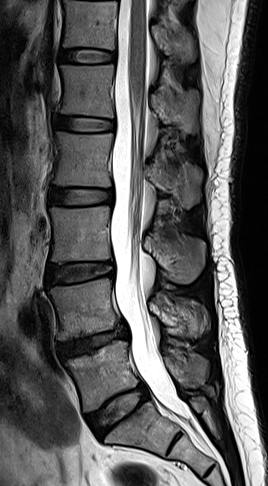
\includegraphics[width=24mm]{mri_sagittal_panel.png}};
\node[cpt] at (16,88) {Sagittal T2, 5 IVD levels};

% pdfcrop'd to its ink, so the 158mm goes to the drawing and not to the
% figure's own margins: every label reads about a third larger than in print.
\node[anchor=north west, inner sep=0] at (46,136)
     {\includegraphics[width=158mm]{hybrid_arch_crop.pdf}};

%% prompts and the per-study output
\node[anchor=base west, font=\fontsize{13}{16}\selectfont]
     at (208,138) {No classifier head, just text prompts.};
\node[anchor=base west, font=\fontsize{10}{13}\selectfont] at (212,131)
     {``\colorbox{slot}{\strut severe} spinal canal stenosis''};
\node[anchor=base west, text=trained, font=\cond\fontsize{10}{12}\selectfont]
     at (208,123) {edit the phrase, get a new label space, no gradient updates};

\node[cpt] at (208,115) {What comes out, for one validation study};
\foreach \x/\h in {208/level, 231/canal, 256/{left foram.}, 281/{right foram.}}
  \node[anchor=base west, text=ink70, font=\cond\fontsize{9.5}{11}\selectfont] at (\x,108) {\h};
\draw[rule, line width=0.2mm] (208,105.5) -- (304,105.5);

\foreach \yy/\lv/\ca/\lf/\rf in {%
    100/{L1-L2}/{Normal/Mild}/{Normal/Mild}/{Normal/Mild},
    95/{L2-L3}/{Normal/Mild}/{Normal/Mild}/{Normal/Mild},
    90/{L3-L4}/{Normal/Mild}/{Normal/Mild}/{Normal/Mild},
    85/{L4-L5}/{Severe}/{Severe}/{Severe},
    80/{L5-S1}/{Normal/Mild}/{Moderate}/{Moderate}}{
  \node[anchor=base west, text=ink, font=\fontsize{9.5}{11}\selectfont] at (208,\yy) {\lv};
  \node[anchor=base west, font=\fontsize{9.5}{11}\selectfont] at (231,\yy) {\ca};
  \node[anchor=base west, font=\fontsize{9.5}{11}\selectfont] at (256,\yy) {\lf};
  \node[anchor=base west, font=\fontsize{9.5}{11}\selectfont] at (281,\yy) {\rf};}
\foreach \x in {231,256,281}
  \node[anchor=base west, text=signal, font=\fontsize{9.5}{11}\selectfont] at (\x,85) {Severe};

%% ---- the rule that splits the page into its two halves
\draw[ink, line width=0.4mm] (16,74) -- (304,74);

%% ===================================================== 2. RESULTS, y 7 to 70
\node[blk] at (16,67) {\textbf{2\quad Results}\, \textcolor{ink70}{\fontsize{13}{15}\selectfont
      Severe recall}\, \textcolor{ink70}{\fontsize{13}{15}\selectfont 12.3\%}\,\arr\,%
      \textcolor{signal}{\fontsize{13}{15}\selectfont\textbf{48.6\%}}%
      \textcolor{ink70}{\fontsize{13}{15}\selectfont , Severe F1 0.152}\,\arr\,%
      \textcolor{ink70}{\fontsize{13}{15}\selectfont\textbf{0.356}}};

%% ---- left: severity distribution
\node[cpt] at (16,60) {Severity distribution, RSNA 2024};
\foreach \yy/\condname/\nm/\mo/\sv/\pct in {%
    47/{spinal canal stenosis}/59.0/5.05/3.23/{4.8},
    37/{left foraminal narrowing}/52.2/12.38/2.76/{4.1},
    27/{right foraminal narrowing}/52.5/12.17/2.62/{3.9}}{
  \fill[waffle]  (16,\yy) rectangle ++(\nm,6);
  \fill[track2]  (16+\nm,\yy) rectangle ++(\mo,6);
  \fill[signal]  (16+\nm+\mo,\yy) rectangle ++(\sv,6);
  \node[anchor=base west, text=ink, font=\cond\fontsize{10}{12}\selectfont]
       at (18,\yy+1.8) {\condname};
  \node[anchor=base west, text=signal, font=\cond\fontsize{10}{12}\selectfont]
       at (16+\nm+\mo+\sv+2,\yy+1.6) {\pct\%};}

\fill[waffle] (16,19) rectangle ++(3,3);
\node[cpt] at (20.5,19.4) {Normal/Mild};
\fill[track2] (44,19) rectangle ++(3,3);
\node[cpt] at (48.5,19.4) {Moderate};
\fill[signal] (68,19) rectangle ++(3,3);
\node[anchor=base west, text=signal, font=\cond\fontsize{10}{12}\selectfont] at (72.5,19.4) {Severe};

% The space under the legend was the one gap left on the page, so it carries
% the experimental setup rather than nothing.
\draw[rule, line width=0.2mm] (16,15) -- (88,15);
\node[anchor=base west, text=ink70, font=\cond\fontsize{9.5}{11}\selectfont] at (16,10.5)
     {Validation 1,942 IVDs from 395 patients, 3 seeds.};
\node[anchor=base west, text=ink70, font=\cond\fontsize{9.5}{11}\selectfont] at (16,6)
     {Both backbones frozen; 66 ms per disc on one RTX 4090.};

\draw[rule, line width=0.2mm] (94,9) -- (94,63);

%% ---- middle: Grad-CAM. Stacked, 44mm, so the pair reads as one comparison
%% on one case rather than two unrelated pictures side by side.
\node[cpt] at (99,60) {Grad-CAM, a Severe spinal canal case};
\node[anchor=south west, inner sep=0] at (99,33)
     {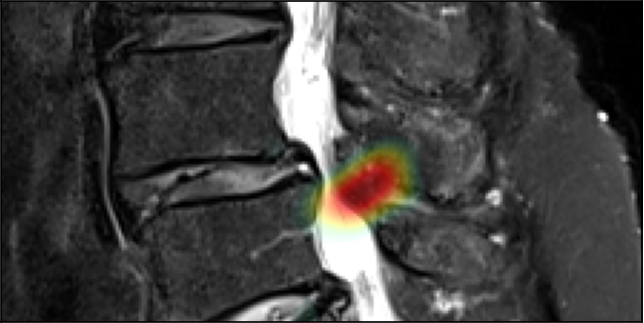
\includegraphics[width=44mm]{gradcam_nocbam.png}};
\node[anchor=south west, inner sep=0] at (99,9)
     {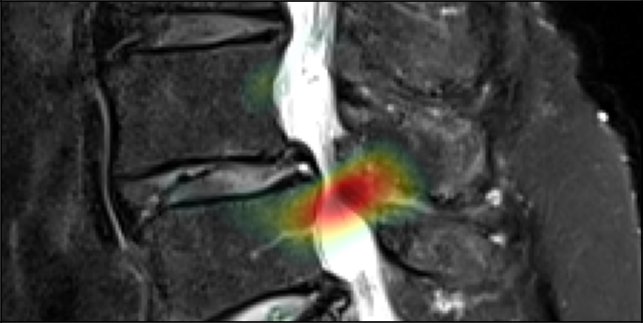
\includegraphics[width=44mm]{gradcam_cbam.png}};
\node[anchor=base west, text=ink70, font=\cond\fontsize{10}{12}\selectfont] at (146,48) {without CBAM};
\node[anchor=base west, text=ink70, font=\cond\fontsize{9.5}{11}\selectfont] at (146,43)
     {heat sits on the};
\node[anchor=base west, text=ink70, font=\cond\fontsize{9.5}{11}\selectfont] at (146,39)
     {vertebral body};
\node[anchor=base west, text=signal, font=\cond\fontsize{10}{12}\selectfont] at (146,24) {with CBAM};
\node[anchor=base west, text=ink70, font=\cond\fontsize{9.5}{11}\selectfont] at (146,19)
     {heat moves onto the};
\node[anchor=base west, text=ink70, font=\cond\fontsize{9.5}{11}\selectfont] at (146,15)
     {narrowed canal};

\draw[rule, line width=0.2mm] (186,9) -- (186,63);

%% ---- right: the full comparison, its heading above the table
\node[cpt] at (191,60) {Every configuration, mean over 3 seeds. Best in each row in bold.};
\node[anchor=base west, text=ink70, font=\cond\fontsize{9.5}{11}\selectfont] at (191,52) {RSNA 2024};
\foreach \x/\h in {243/{SpineNetV2}, 263/{CBAM}, 281/{Multim.}, 299/{Hybrid}}
  \node[anchor=base east, text=ink70, font=\cond\fontsize{9.5}{11}\selectfont] at (\x,52) {\h};
\draw[rule, line width=0.2mm] (191,49.5) -- (304,49.5);

% Bold marks the best cell in the row; the accent still belongs to the Severe
% class alone, so only the two Severe rows carry it. Mean Accuracy is the row
% the hybrid loses, and it is printed exactly like the rows it wins.
\foreach \yy/\m/\a/\b/\c/\d in {%
    44.5/{Mean Accuracy \%}/{\textbf{81.0}}/{69.5}/{71.2}/{72.4},
    39.9/{Mean F1 macro}/{0.420}/{0.477}/{0.482}/{\textbf{0.527}},
    35.3/{Mean Recall macro}/{0.412}/{0.531}/{0.532}/{\textbf{0.592}}}{
  \node[anchor=base west, text=ink, font=\fontsize{9.5}{11}\selectfont] at (191,\yy) {\m};
  \node[anchor=base east, font=\fontsize{9.5}{11}\selectfont] at (243,\yy) {\a};
  \node[anchor=base east, font=\fontsize{9.5}{11}\selectfont] at (263,\yy) {\b};
  \node[anchor=base east, font=\fontsize{9.5}{11}\selectfont] at (281,\yy) {\c};
  \node[anchor=base east, font=\fontsize{9.5}{11}\selectfont] at (299,\yy) {\d};}

\foreach \yy/\m/\a/\b/\c/\d in {%
    30.7/{Severe Recall}/{0.123}/{0.288}/{0.316}/{\textbf{0.486}},
    26.1/{Severe F1}/{0.152}/{0.262}/{0.268}/{\textbf{0.356}}}{
  \node[anchor=base west, text=signal, font=\fontsize{9.5}{11}\selectfont] at (191,\yy) {\m};
  \node[anchor=base east, font=\fontsize{9.5}{11}\selectfont] at (243,\yy) {\a};
  \node[anchor=base east, font=\fontsize{9.5}{11}\selectfont] at (263,\yy) {\b};
  \node[anchor=base east, font=\fontsize{9.5}{11}\selectfont] at (281,\yy) {\c};
  \node[anchor=base east, text=signal, font=\fontsize{9.5}{11}\selectfont] at (299,\yy) {\d};}

\draw[rule, line width=0.2mm] (191,22.5) -- (304,22.5);
\node[anchor=base west, text=ink70, font=\cond\fontsize{9.5}{11}\selectfont] at (191,18)
     {SPIDER, supervised transfer, 8 unseen labels};
\node[anchor=base west, text=ink, font=\fontsize{9.5}{11}\selectfont] at (191,12.5) {Mean F1 macro};
\foreach \x/\v in {243/{0.646}, 263/{0.619}, 281/{0.613}, 299/{\textbf{0.653}}}
  \node[anchor=base east, font=\fontsize{9.5}{11}\selectfont] at (\x,12.5) {\v};
\node[anchor=base west, text=ink70, font=\cond\fontsize{9.5}{11}\selectfont] at (191,6)
     {Zero-shot, no SPIDER training: disc bulging F1 0.613, spondylolisthesis 0.028};

\end{tikzpicture}
\end{document}
